% !TEX TS-program = pdflatexmk
% !BIB TS-program = bibtex

\documentclass[12pt, a4paper, twoside]{book}
\usepackage{import}
\subimport{../}{preamble}
\ExecuteBibliographyOptions{articletitle=false}
\standalonetrue
\onehalfspacing
\begin{document}

\begin{singlespace}
\chapter{Outlook and Conclusions}
\end{singlespace}

%\AddToShipoutPictureBG*{ \AtPageUpperLeft{ \put(0,-240)
%{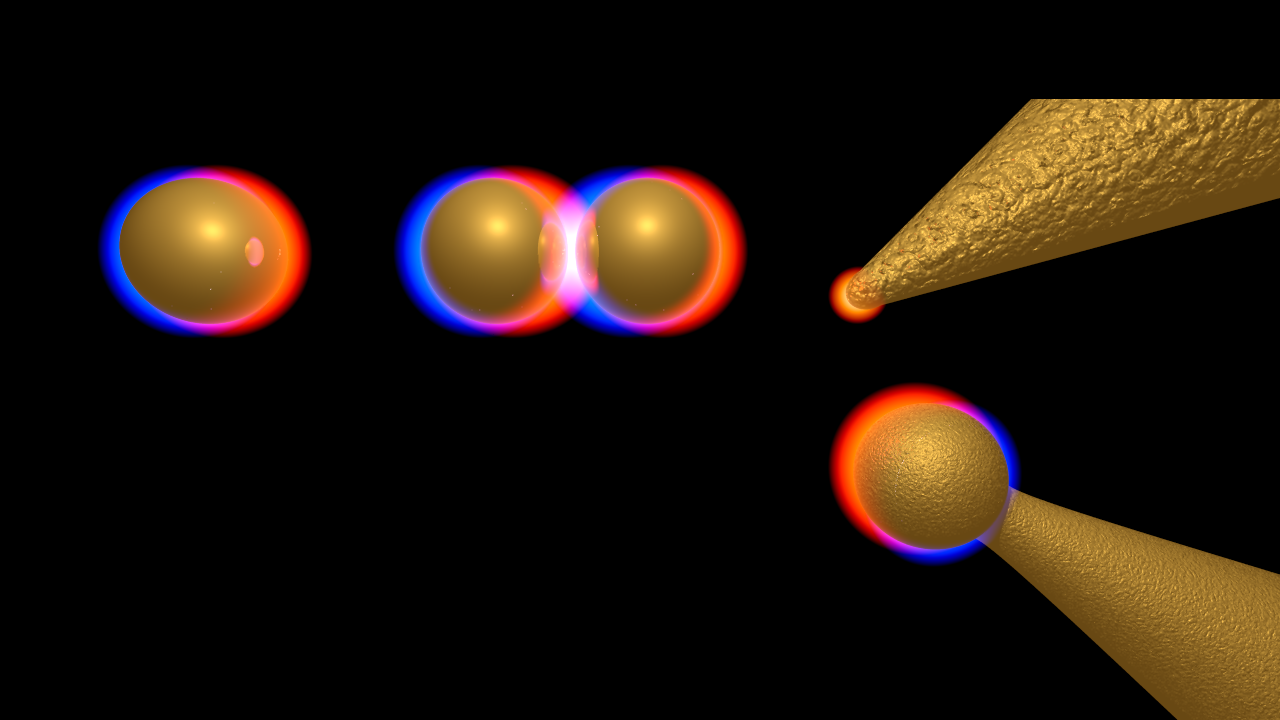
\includegraphics[width=\paperwidth, clip=true, trim=0 80 0 100]{figures/chapter_cover.png}}
%}}

% Project overview
This thesis has focussed on the understanding and application of tips for plasmonics, with the aim to use tips to further understand the recently revealed sub-nm regime of plasmonic coupling. To achieve this difficult task one must obtain greater understanding of the underlying physics defining the excitation of surface plasmon polaritons and the limiting factors governing what can be observed experimentally. From there plasmon coupling can be probed by bringing two opposing tips together {\color{red}in ambient conditions} while watching the spectra change under the influence of tunnelling currents. To succeed in developing a robust method of measuring plasmon coupling, this project required the both careful design and understanding of the experimental setup and the plasmonic tips used.

% Review of test rig design chapter
The study of tips necessitated the design and construction of a microscope capable of combining the function and stability of two opposing AFM devices with a platform for broadband dark-field spectroscopy. The design behind the microscope has been discussed at length and its performance demonstrated and quantified.
% Review of experimental procedures chapter
The experimental techniques developed to discern the plasmonics of both individual and coupled nanostructures and performed using this setup have been discussed.  This project has shown how hyperspectral imaging can be used to extract more information than a single image or spectrum can provide. This technique has been used to spatially probe localised surface plasmons.
By applying both hyperspectral imaging and scanning capacitance microscopy to the electrically-contacted AFM tips they can be aligned in three dimensions to both the incident illumination and to each other, resulting in a greater structure reminiscent of a bow-tie nanoantenna or nanoparticle dimer. At this point the dynamical coupling between plasmons can be optically probed using correlated measurements of scattering, electronics and force to discern the nanoscale behaviour.

% Review of why spherical tips are necessary
The lack of observation of far-field plasmonic behaviour in sharp Au tips, despite their prominence in many near-field enhancing techniques, motivates the use of nanostructured tips. Nanostructuring aimed to transfer some of the well-known antenna-like properties of plasmonic nanostructures into the tip probe form factor. Spherical tips, the simplest form of nanostructuring, are developed using pulsed electrodeposition, and further compared with commercially available spherical tips.
% Characterisation of tips
Optical characterisation of both kinds of spherical tips clearly showed that the plasmonic behaviour of the far-field antenna modes in spherical nanoparticles is imparted onto the spherical tip. The creation of these localised surface plasmon states allows far-field light to be efficiently transmitted to the nanoscale, a process not possible{\color{red}, or not efficient,} with a sharp morphology. The existence of these modes is important as they limit what can be experimentally observed and has significant implications regarding the way tips can be used for near-field optics. In particular, the side-illumination geometry becomes applicable once again after being surpassed by the evanescent wave coupling geometry required to excite planar SPPs and sharp tip LSPs. This hinges on there being a readily available supply of plasmon antenna tips to fuel near-field microscopes and progress the optimisation of the nanotip antenna geometry. For this reason ready availability of these plasmonic antenna probes is an important issue to address.

% Fabrication of tips
The simple electrochemical method of exploiting the sharpness of a metallic tip to successfully fabricate spherical AuNP-on-Pt AFM tips provided a useful method for acquiring plasmonic antenna tips but without exacting the desired amount of control on the plasmon properties to fully tailor experiments. In its current form it provides a fast way to nanostructure tips but does not have the reproducibility required to properly manufacture such tips with industrial quality levels. Further work is required to hone the morphology, and hence plasmonic response, of fabricated spherical tips. With such a large parameter space to explore it was unfeasible to complete such work whilst simultaneously developing the microscope, experimental procedures and understanding of the plasmons and plasmon coupling in individual sharp and spherical tips.

\section{Applications of Spherical Tips}

% Applications of spherical tips outside of plasmon coupling studies
Not only can spherically nanostructured tips be used to fundamentally probe the interaction between coupled plasmons but they have shown promise as near-field enhancing probes with the capability for far-field plasmon excitation. This plasmon contribution greatly adds to the overall near-field enhancement despite the loss of the sharpness and its lightning rod enhancement. The overall result of the added plasmon component is an improvement in the Raman response when using spherical tips over the more traditional sharp morphology when using a side-illumination geometry.

\section{Follow-up Experiments in the Tunnelling Regime}

% Gap mode coupling
By bringing two plasmonic tips together gap plasmon coupling can be studied dynamically, with the antenna modes mitigating/managing the near-field to far-field energy conversion.
% Things still to do
This project leaves at a pivotal point at which atomic-scale morphology and quantum effects have been shown to strongly influence the plasmons confined to a sub-nm gap between metallic surfaces.
Many questions still remain unanswered for both classical and quantum coupling regimes.
% Different humidity
In the quantum regime the effect of humidity has yet to be addressed. Compared to experiments performed in vacuum, does humidity change the length of the tunnelling regime or position of resonances? The fact that water is always present to some extent in ambient conditions would suggest that humidity may change the amount of adhesion between tips, or the rate of redshift when transitioning between a gaps in air to gaps in water but the plasmonics are so confined in the sub-nm regime that they can be considered to be in a complete water environment regardless of humidity.

% Different conduction mechanisms
While there is little phenomenological dependence on the conduction mechanism it can still be important to identify the specific mechanism in a given system. Exploring the idea of quantum tunnelling vs. molecular tunnelling with conductive molecules during the different phases of making contact is also possible in this experiment. There is no guarantee without further measurements of conductance at each point in a scan (such as temperature dependence, $dI/dV$, etc.) that quantum tunnelling is the only charge transfer event taking place. Even within electron tunnelling there is no distinction made between quantum (vacuum) tunnelling and molecular tunnelling.  Tunnelling through different media have different rates due to changes to the barrier work function. The decay rate in vacuum (\SI{2.9}{\per\angstrom}) is much greater than the decay rate in molecules (0.8--\SI{0.9}{\per\angstrom} and 0.1--\SI{0.3}{\per\angstrom} for saturated and unsaturated molecules, respectively) \cite{tan2014}, hence the signatures of tunnelling plasmonics are seen at larger interparticle separations when molecules bridge the gap \cite{tan2014, benz2014}.

% Different biases
The bias during conduction also plays a role \cite{} and to date only biases with $V\sim\orderof{\textrm{mV}}$ have been tried to maintain acceptable signal levels. Lower biases could improve the reproducibility of the theoretical case of only an optical driving field with no mixing component from the d.c. bias. Larger biases could potentially satisfy $eV>h\nu$ in the visible and NIR meaning electrical excitation of gap modes.
% Attempting electrical excitation in a dynamic system.
One of the most promising directions one could take dual tip spectroscopy is to attempt electrical excitation of gap modes, using stiff ($k=\SI{40}{N\per\metre}$) probes to overcome the increased electrostatic pull between tips. The effect of the tunnelling current on different tip geometries in a dynamic dimer configuration could then be probed using electrically-induced light scattering. This would mean that only the tunnelling regime could be probed but with a background-free scattering signal. Given the previous uses in the literature the approach may also work with sharp tips as there is no strict requirement for efficient coupling to far-field excitation.

% Tip to mirror experiments
Some initial experimentation has been done attempting to couple the plasmons in a spherical Au tip with its mirror charge in a Au mirror (the backside of another Au AFM cantilever). This presents a potentially simple method for dynamically measuring the plasmonic properties of particles coupled with their image charge, a topic currently receiving much attention \cite{mertens2013, benz2014}. One difficult however is the ability to illuminate the particle and gap, as well as collecting the scattered light, since the cantilever blocks a significant portion of the beam.

How does spectra respond to dynamic $xy$ scans at fixed $z$?
There is also the potential for different tip geometries, such as rounded tips, which have the potential to change the way in which we observe the quantum regime \cite{}.

\section{Concluding Remarks}

\ifstandalone
\begin{singlespace}
\fontsize{8pt}{1em}\selectfont
\printbibliography[notcategory=fullcited]
\end{singlespace}
\fi

\end{document}